\subsection*{Project Description}
The purpose of this project is to model the ROVU system which is composed of multiple robots, a control station and operators controlling said station. The robot rovers are supposed to carry out missions which are sent out by an operator through the control station. To carry out these missions the robot will have to calculate a strategy while taking the current procedure of rewarding points into account so as to acquire the most amount of points possible during the duration of the mission.\newline
After modelling the system, a working version of the system will be implemented within the provided simulation environment. So as to show that the model created during the project work may meet the requirements in practice.


\subsubsection*{Choosing the Use Cases}
While rendering our idea for the project and our domain model, we also defined a set of use cases. We then prioritised them, and picked the six most vital ones.
The six use cases which have been chosen as the most critical part of the system are as follows.
\begin{itemize}
    \item Assign Mission
      \begin{itemize}
          \item The assigning of missions is one of the most basic functionalities of the system. It allows the operator to impose their wishes of where the robot is supposed to go and through these points a strategy can then be calculated.
      \end{itemize}
    \item Calculate Strategy
      \begin{itemize}
          \item The calculation of strategy is necessary for having the robot make the decision of which route to take when visiting the points laid out by the assigned mission. This use case is dependent on the 'Reward Points' use case since the robot will need the point distribution in order to make the "best" possible strategy decition 
      \end{itemize}
    \item Navigate to Point
     \begin{itemize}
         \item This is a critical part of the system in the sense that it fulfils the most basic functionality of our robot system. To be able to execute missions and gather points a robot must be able to navigate to the points which have been selected by the operator.
     \end{itemize}
    \item Reward Points
      \begin{itemize}
          \item This use case ties into the 'Calculate Strategy' use case since to be able to calculate the best possible strategy for how to visit points, a robot should be presented with "benefits" with the aim to have the robot take the best possible route according to the reward procedure which has been established.
      \end{itemize}
    \item Update Procedure
      \begin{itemize}
          \item As mentioned above this use case is necessary for both the 'Calculate Strategy' and 'Reward Points' use cases. This procedure decides on how many points will be awarded to robots which are present within a certain area within a certain time-frame(every 20 seconds). 
      \end{itemize}
    \item Handle Failure
      \begin{itemize}
          \item In the case of a fault occurrence which hinder robot functionality or is likely to cause the robot to be subjected to damage, a fault handling procedure should be established. This could be anything from trying to restart subsystems to basically just shutting down and awaiting pick-up.
      \end{itemize}
\end{itemize}
\subsection*{Use Cases in Detail}
In this section we describe the use cases we prioritised, in more detail and according to the template provided.
\newline

Assign Mission
\begin{itemize}
    \item Responsible: Sebastian
    \item Controller: William
    \item Actor: Operators, Control Station
    \item Goal: The control station receives the mission assigned by the operator
    \item Description: The operator designs a mission - a set of points for the robot to visit - then sends it off to the control station through the interface. This use-case triggers the Calculate Strategy use case in the control station.
\end{itemize}

Calculate Strategy
\begin{itemize}
    \item Responsible: Victor
    \item Controller: Sebastian
    \item Actor: Robot
    \item Goal: Get a route which completes the mission in the optimal order.
    \item Description: Upon receiving a set of points, the robot compares their coordinates to its knowledge of its environment - any well known physical or logical areas, and their respective physical obstacles, then calculates the optimal order and route for the mission execution.
\end{itemize}
Navigate to Point
\begin{itemize}
    \item Responsible: Snezhina
    \item Controller: Victor
    \item Actor: Robot
    \item Goal: Reach the geographical point.
    \item Description: Once the mission has been broken down into steps, the robot executes them in sequence. Each step navigation is triggered by the step being reached in the list. After this, the robot calculates the angle of its next movement, the distance it needs to go, and performs the navigation. On the way, it avoids obstacles with help of different
kinds of sensors and it's knowledge about the surroundings.
\end{itemize}
Reward Points and Update Interface
\begin{itemize}
    \item Responsible: Svante
    \item Controller: Snezhina
    \item Actor: Control Station
    \item Goal: Rewarding the points that have been acquired and show the operator that this indeed is the case. 
    \item Description: The points are calculated so now the Control Station just needs to reward them to the Operator and doing so by changing the interface so that it is shown that points have been rewarded.
\end{itemize}
Update Procedure
\begin{itemize}
    \item Responsible: Philip
    \item Controller: Svante
    \item Actor: Control Station
    \item Goal: Switch the current point calculation procedure according to their definition.
    \item Description: In order to fairly reward points based on the robots' location within physical and logical areas, two separate procedures are used. When the control station realises the conditions for switching the reward procedure are met, it signals the robots in order for them to know that the procedure was updated.
\end{itemize}
Handle Failure
\begin{itemize}
    \item Responsible: William
    \item Controller: Philip
    \item Actor: Robot
    \item Goal: Handle any failure that occurs to the Robot.
    \item Description: In order the not shut down, the Robot must handle when something is wrong for example, a wheel is broken and there is no guarantee that the connecting between the Control Station and the Robot is down so the Robot has handle the problem itself.
\end{itemize}

\newpage
\begin{figure}
    \centering
    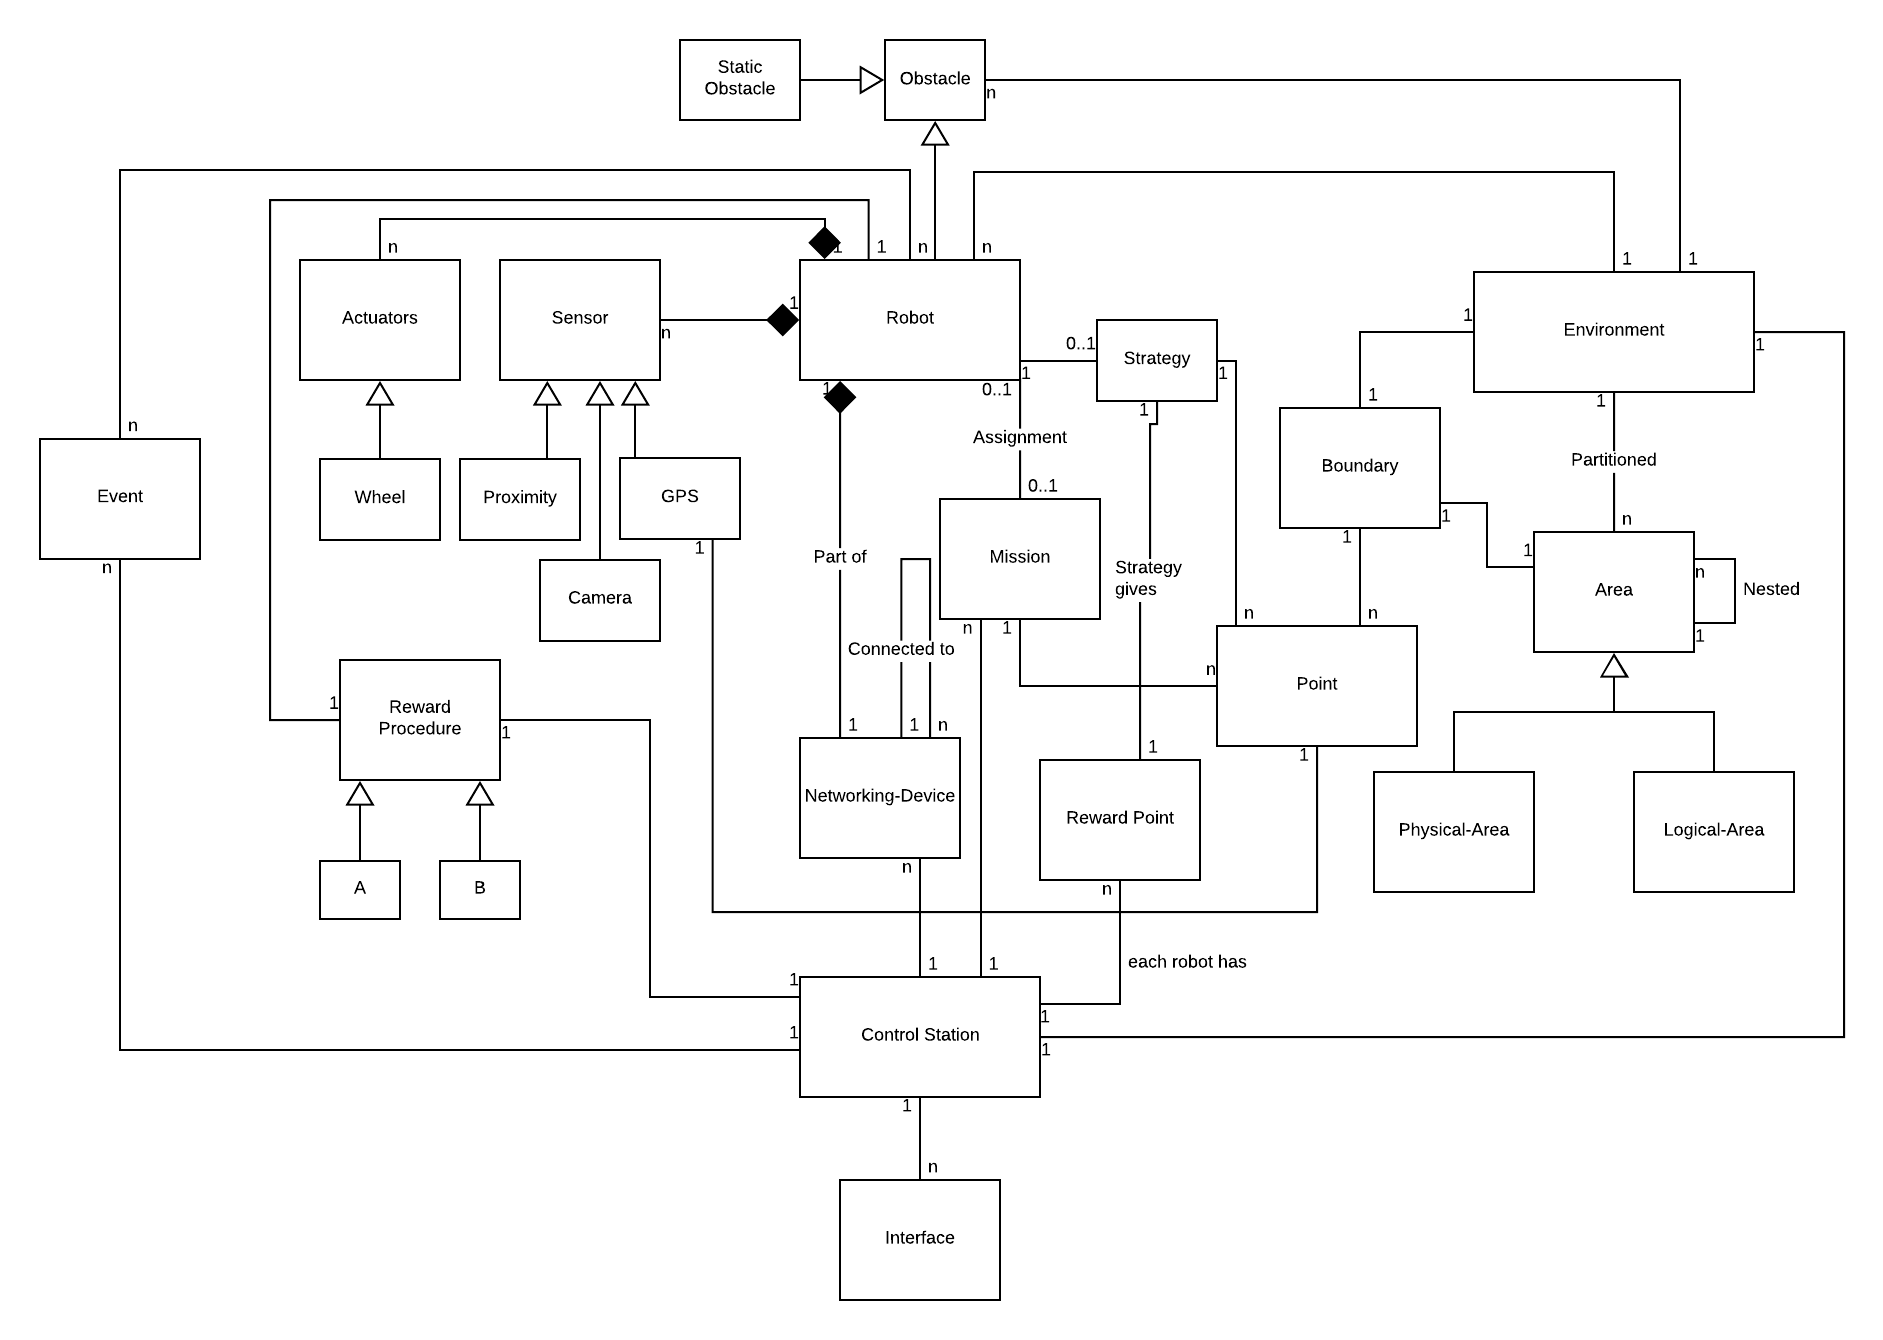
\includegraphics[width=22cm, angle=-90]{docs/domain/model.png}
    \caption{Domain Model}
    \label{fig:domain}
\end{figure}

\subsection*{Domain description}
In our system we consider rovers to be instances of robots and thus have the generalisation 'robots' in our domain. 
The robot is in our system also considered to be a type of obstacle. The assumption which we have made is that the only dynamic obstacles present in the environment is other robots roaming the areas while the rest of the obstacles are static.\newline
The environment is made up of a set of areas for-which the areas can be either logical areas and the physical areas. These areas have boundaries which act as separators and limiters for the different areas, while the environment boundary is the limiting scope of the entire set of areas.\newline
The control station acts as the medium between the operator and the robots. It is connected to the robots through a networking device, and through this station the operator can send 'commands' which influence the behaviour of the robot which it has been sent to. While the control station does have the ability to send these 'commands' to the robots we still consider the robot responsible for its own fault handling, e.g if a fault occurs it should have a list of different reactions according to the situation.\newline 
A robot has a singular reward procedure to take into account when calculating a strategy. Strategies are calculated ways to finish a mission while earning as many points as possible, while still fulfilling every requirement of a mission.
A mission includes several points that the rover has to visit, and may involve other restrictions such as a time limit. A robot also has actuators and sensors that provide the physical ability to execute strategies, as well as the data required to calculate them.

\newpage
\begin{figure}
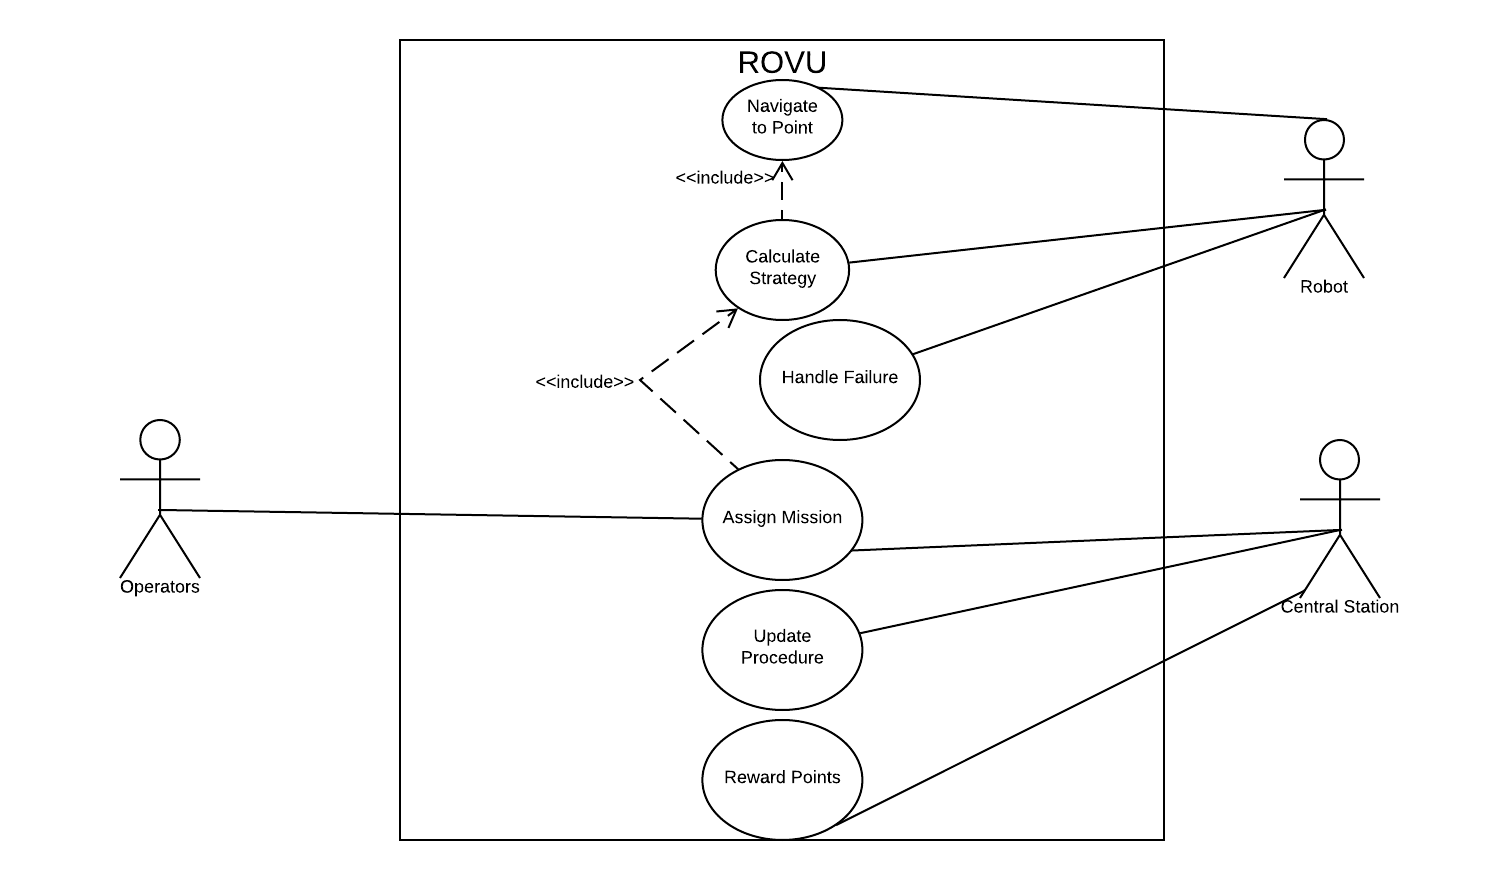
\includegraphics[width=22cm, angle=-90]{docs/domain/use_cases/use_case_diagram.png}
\end{figure}

